\chapter{Evaluación y métricas}\label{cap.evaluacion}

En este capítulo se explican las distintas métricas que se calculan tras pasar el conjunto de \textit{test} por la red previamente entrenada, permitiendo obtener una medida objetiva de la bondad de dicha red. Además se realiza un análisis en profundidad del código Python desarrollado para tal fin y se hace una interpretación sobre los gráficos y resultados que arroja dicho código al terminar la ejecución.

\section{Métricas}

A continuación se describen, de forma teórica, las distintas métricas que se emplean para evaluar el rendimiento de las redes estudiadas. La comparación de estas medidas objetivas ha permitido extraer diversas conclusiones sobre algunos parámetros como el número de muestras utilizadas para entrenar, la complejidad de la dinámica o la distancia temporal a la que se quiere predecir.

\begin{description}
\item[Distancia entre píxeles] \hfill 
\vspace{10pt}
\\
La medida que se utiliza como base del error cometido en cada una de las predicciones es la distancia entre el píxel predicho y el real, haciendo uso de la distancia Euclídea\footnote{\url{https://en.wikipedia.org/wiki/Euclidean_distance}} cuya fórmula, en dos dimensiones, es:  
$$error = d(p,q) = \sqrt{(p_1 - q_2)^2 + (p_1 - q_2)^2}$$\\
\vspace{10pt}
\\
Además, para un mayor análisis más profundo, se calcula esta distancia desglosada en cada una de las dimensiones de la imagen, \textit{x} e \textit{y}, simplemente mediante la diferencia en términos absolutos del valor en dichas coordenadas:
$$error_{dim} = d(p_{dim}, q_{dim}) = |p_{dim} - q_{dim}|$$
Esta distancias son consideradas como el error absoluto cometido en el plano general de la imagen y sus dimensiones \textit{x} e \textit{y}, y sobre él se calculan tanto el error relativo como los distintos estadísticos que permitan analizar de una forma más completa la bondad de la red.

\vspace{10pt}

\item[Error relativo] \hfill 
\vspace{10pt}
\\
El error absoluto puede dar una visión incompleta sobre el fallo que se ha cometido: no es lo mismo desviarse una distancia de 5 píxeles en una imagen de 5x5 que en una de 1920x1080 y por ello se hace uso del error relativo\footnote{\url{https://en.wikipedia.org/wiki/Approximation_error}}. Este concepto normaliza el error absoluto cometido con el máximo que es posible cometer, haciendo uso de la siguiente fórmula:
$$\eta = \frac{\epsilon}{|\upsilon|}$$
En el caso de las imágenes, el máximo error a cometer es la mayor distancia que existe dentro de la misma que, al tratarse de un cuadrilátero, se corresponde con la diagonal cuyo valor se obtiene de la siguiente manera:
$$|\upsilon| = D = \sqrt{h^2 + w^2}$$
donde \textit{h} y \textit{w} son la altura y anchura de la imagen respectivamente.

Este error se suele representar de forma porcentual, por lo que el valor calculado se multiplica por 100 para su expresión como porcentaje:
$$\delta = \eta * 100\%$$

Con el cálculo de este error se consigue normalizar la medida para poder comparar imágenes de distinto tamaño y tener una idea más realista del fallo que se está cometiendo.

\vspace{10pt}

\item[Estadísticos] \hfill 
\vspace{10pt}
\\
Con ambos errores calculados para cada una de las muestras, se obtiene una serie de estadísticos representativos sobre el vector de errores que permite la comparación entre redes y la extracción de conclusiones. A continuación se describen los estadísticos considerados y su forma de representación.

\begin{itemize}
    \item \textbf{Máximo:} Se trata del error máximo cometido sobre todas las muestras analizadas. Mediante este valor se obtiene la muestra en la que más distancia existe entre la posición real y la predicha, que será representada en el gráfico final.
    \item \textbf{Media:} Se calcula la media de los vectores de error resultantes, absoluto y relativo, para obtener un único valor que permita hacer comparaciones rápidas.
    \item \textbf{Histograma:}\footnote{\url{https://en.wikipedia.org/wiki/Histogram}} Es un gráfico de barras que enfrenta la frecuencia con la que se comete un error con el valor del mismo, agrupado en intervalos para una representación más compacta.
    \item \textbf{\textit{Boxplot}:}\footnote{\url{https://matplotlib.org/3.3.1/api/_as_gen/matplotlib.pyplot.boxplot.html}} Se trata de un diagrama de caja y bigotes en el que la caja representa los cuartiles y las líneas que se extienden desde ella indican variabilidad fuera de los cuartiles superior e inferior. Por otro lado, los valores atípicos se representan como puntos individuales dispersos por el eje vertical de la caja.
\end{itemize}

Estos elementos se combinan en una única imagen dividida en cuatro regiones: una para el histograma del error absoluto, otra para el del relativo, una tercera para el \textit{boxplot} y la última con información de la media y el máximo; que permite representar de una forma resumida y clara toda la información referente al rendimiento de la red, para una posterior comparación entre redes.
\vspace{10pt}
\end{description}

Para el cálculo de todas las medidas explicadas y la obtención de la imagen final se ha desarrollado una herramienta en Python sobre la que se profundiza en la siguiente sección.

\section{Herramienta de evaluación}

En la Figura~\ref{fig.flujo_test} se puede visualizar el flujo que sigue el código para la evaluación de una red concreta con un conjunto de \textit{test} determinado.

\vspace{10pt}
\begin{figure}[H]
    \begin{center}
        \begin{tikzpicture}[node distance=2cm]
            \node (ld) [treenodelong] {Lectura de datos};
            \node (net) [treenodelong, below of=ld] {Carga de la red};
            \node (pred) [treenodelong, below of=net] {Predicción};
            \node (trans) [treenodelong, below of=pred] {Transformación de posiciones};    
            \node (calc) [treenodelong, below of=trans] {Cálculo de métricas};
            \node (pres) [treenodelong, below of=calc] {Presentación de resultados};
            
            \draw [arrow] (ld) -- (net);
            \draw [arrow] (net) -- (pred);
            \draw [arrow] (pred) -- (trans);
            \draw [arrow] (trans) -- (calc);
            \draw [arrow] (calc) -- (pres);
        \end{tikzpicture}
        \caption{Diagrama de flujo del evaluador.}
	    \label{fig.flujo_test}
	\end{center}
\end{figure}

En este caso, el programa sigue un flujo muy sencillo y lineal que permite obtener, al final del mismo, una serie de valores asociados a las métricas explicadas anteriormente así como los gráficos que permiten resumir toda la información de una forma más visual, facilitando la labor de comparación.\\

En primer lugar se realizan las operaciones de lectura del conjunto de \textit{test} y carga de la red en memoria, cuyas rutas se obtienen del fichero de configuración correspondiente, para posteriormente pasar por la red los datos y se obtener las predicciones.\\
\vspace{20pt}
\\
Las posiciones que se obtienen a la salida de la red tienen un formato que no se ajusta con el que tienen las reales, con las que se hará la comparación, por lo que es necesario realizar una transformación previa. Esta operación dependerá del tipo de datos, modelados o crudos, que se estén tratando pues el problema se afronta de manera distinta en función de ello, según se explica en el los Capítulos~\ref{cap.redes3dmod}~y~\ref{cap.redes3dcrud}.\\
Cuando se está tratando con datos modelados se hace un trabajo de regresión, por lo que la salida de la red es un par de valores que coincide con el de la posición estimada y la única acción a realizar es el redondeo de la cifra para obtener un número entero. El procesamiento en el código queda de la siguiente manera:
\vspace{10pt}
\begin{lstlisting}[frame=single]
  p = np.round(p).astype(np.float64)
  predict_pos.append(p)
\end{lstlisting}
Si se está trabajando con muestras en crudo, el problema de predicción se afronta como un problema de clasificación en el que la salida es un vector de longitud \textit{hxw}, con la clase asociada a la posición. En este caso se redimensiona el vector de salida al del tamaño de la imagen y se obtiene la posición del píxel activo de la siguiente forma:
\vspace{10pt}
\begin{lstlisting}[frame=single]
  p = p.reshape(dim)
  predict_pos.append(np.unravel_index(p.argmax(), p.shape))
\end{lstlisting}

Una vez obtenidas las posiciones predichas y reales en el mismo formato se procede a el cálculo de las métricas mediante el siguiente proceso:

\begin{enumerate}
    \item Se calcula la distancia de cada elemento entre la posición real y la estimada.
    \item Se calculan los errores absolutos y relativos de cada muestra en el plano de la imagen y las dimensiones \textit{x} e \textit{y}.
    \item Se calculan los estadísticos sobre cada uno de los errores obtenidos.
    \item Se crean los histogramas de los errores absoluto y relativo sobre el total de la imagen.
    \item Se obtiene y representa la muestra de máximo error sobre el total de la imagen, tanto absoluto como relativo.
    \item Se crea el \textit{boxplot} para los errores sobre los tres planos: total de la imagen, dimensión \textit{x} y dimensión \textit{y}.
\end{enumerate}

Finalmente, con todas las medidas calculadas y los gráficos creados se almacenan en dos formatos distintos:
\begin{itemize}
    \item El fichero \textit{error}\_\textit{result.txt} almacena para cada una de las muestras el número de la misma, la posición real, la posición predicha y los errores, absoluto y relativo, que se han cometido en la misma.
    \item Una imagen que aúna cuatro gráficos significativos: los histogramas de los errores absolutos y relativos, el \textit{boxplot} de ambos errores y la representación de la muestra de máximo error. En la Figura~\ref{fig.test_example} se presenta un ejemplo de esta imagen resumen.
    \begin{figure}[H]
		\begin{center}
			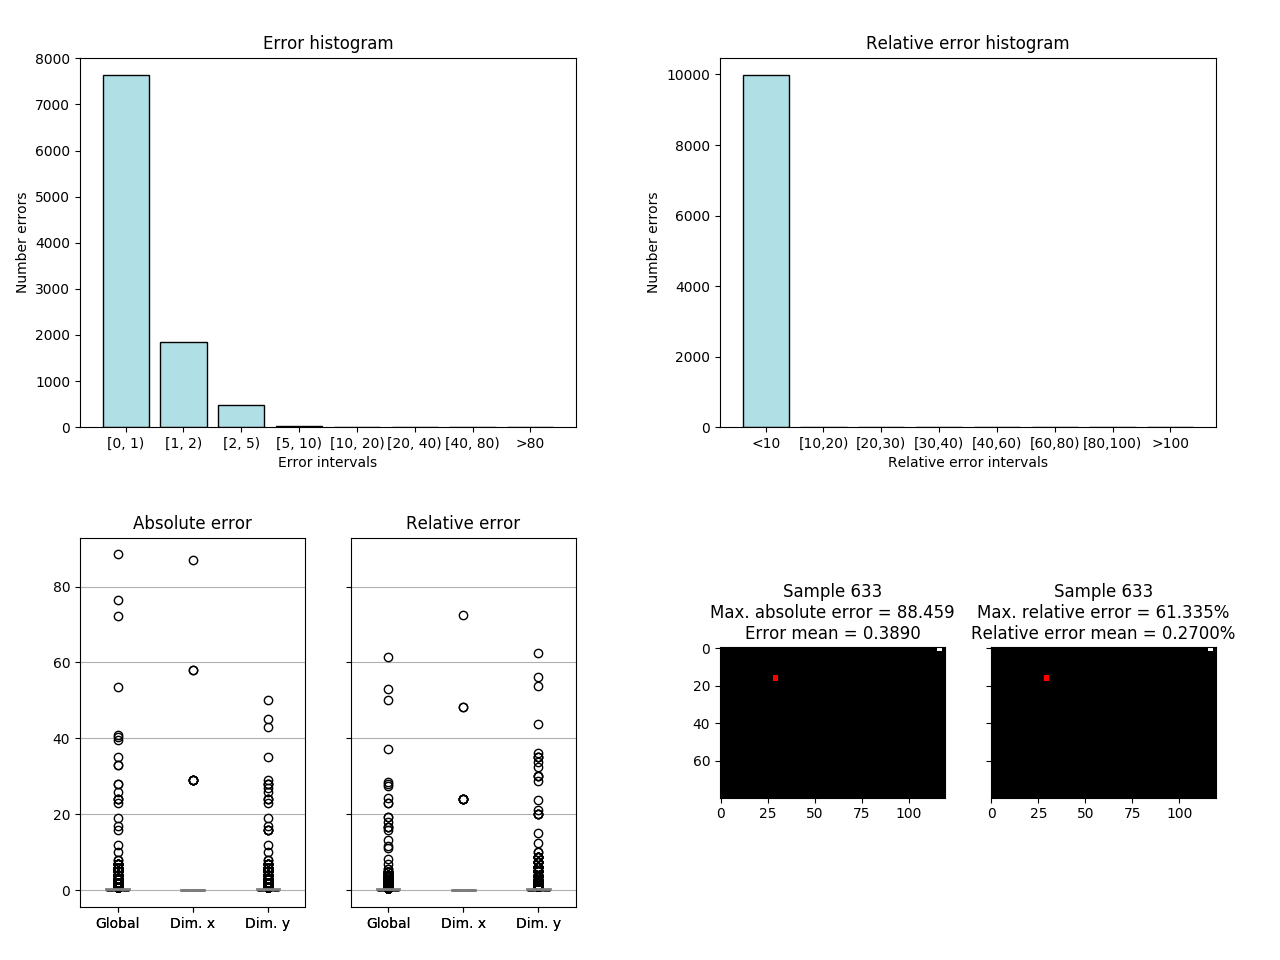
\includegraphics[width=0.9\textwidth]{Memoria-TFM/figures/test/error_stats_example.png}
			\caption{Ejemplo de gráficos de error.}
			\label{fig.test_example}
		\end{center}
    \end{figure}
    \vspace{-10pt}
\end{itemize}

Con estos resultados se dispone de una forma objetiva de comparación entre las redes a estudiar que permita extraer conclusiones sobre distintos aspectos de las mismas.